\documentclass[a4paper, 12pt]{article}

\usepackage[margin=2cm]{geometry}
\usepackage[T2A]{fontenc}
\usepackage[utf8]{inputenc}
\usepackage[russian]{babel}
\usepackage{multicol}
\usepackage{graphics}
\usepackage{rotating}
\usepackage{diagbox}
\usepackage{fancyhdr}
\usepackage{multirow}
\usepackage{cmap}
\usepackage{gensymb}

\usepackage{caption}
\captionsetup{labelsep=period}

\usepackage{float}

%\setlength{\parindent}{0em}
%\setlength{\parskip}{1em}

\usepackage{amsmath, amsfonts, amssymb, amsthm, mathtools}
\usepackage{icomma}


\begin{document}
	\begin{titlepage}
		\begin{center}
			\large\textbf{Московский Физико-Технический Институт}\\
			\large\textbf{(государственный университет)}
			\vfill
			\huge\textbf{Лабораторная работа 2.1.6\\ Эффект Джоуля-Томсона}\\
			\ \\
			\large Овсянников Михаил Б01-001\\
			\vfill
			\large ФРКТ\\
			\large Долгопрудный, 2021
		\end{center}
	\end{titlepage}
	\newpage
	\pagestyle{fancy}
	\setcounter{page}{2}
	\fancyfoot[c]{\thepage}
	\fancyhead[L] {Работа 2.1.6}
		\indent	{\large \textbf{Работа 2.1.6}}
		\\ 
		\\
		\indent \textbf{\LARGE 		Эффект Джоуля–Томсона}
		\\
	
	\textbf{Цель работы:} 
	1) определение изменения температуры углекислого газа при протекании через малопроницаемую перегородку при разных начальных значениях давления и температуры; 2) вычисление по результатам опытов коэффициентов Ван-дер-Ваальса «a» и «b».
	\\ 
	\\
	\indent \textbf{В работе используются:} трубка с пористой перегородкой; труба Дьюара; термостат; термометры; дифференциальная термопара; микровольтметр; балластный баллон; манометр.
	\\
	\\
	\indent Эффектом Джоуля–Томсона называется изменение температуры газа, медленно проте кающего из области высокого в область низкого давления в условиях хорошей тепловой изоляции. В разреженных газах, которые приближаются по своим свойствам к идеальному газу, при таком течении температура газа не меняется. Эффект Джоуля–Томсона демонстрирует отличие исследуемого газа от идеального.
	
\indent В работе исследуется изменение температуры углекислого газа
при медленном его течении по трубке с пористой перегородкой (рисунок 1). Трубка 1 хорошо теплоизолирована. Газ из области повышенного давления $P_{1}$ проходит через множество узких и длинных каналов пористой перегородки 2 в область с атмосферным давлением $P_{2}$. Перепад давления $\Delta P = P_{1} - P_{2}$ из-за большого сопротивления каналов может быть заметным даже при малой скорости течения газа в трубке. Величина эффекта Джоуля–Томсона определяется по разности температуры газа до
и после перегородки.

\indent Рассмотрим стационарный поток газа между произвольными сечениями $I$ и $II$ трубки (до перегородки
и после нее). Пусть, для определенности, через трубку прошел 1 моль углекислого газа; $\mu$ — его
молярная масса. Молярные объемы газа, его давления и отнесенные
к молю внутренние энергии газа в сечениях $I$ и $II$ обозначим соответственно $V_{1}, P_{1}, U_{1}$ и $V_{2}, P_{2}, U_{2}$.Для того чтобы ввести в трубку объем $V_{1}$, над газом нужно совершить работу $A_{1} = P_{1}V_{1}$. Проходя через сечение $II$, газ сам совершает работу $A_{2} = P_{2}V_{2}$, Так как через боковые стенки не происходит ни обмена теплом, ни передачи механической энергии, то

\begin{equation}
	A_{1} - A_{2} = \left(U_{2} + \frac{\mu v_{2}^2}{2}\right) - \left(U_{1} + \frac{\mu v_{1}^2}{2}\right)
\end{equation}

В уравнении (1) учтено изменение как внутренней (первые члены в
скобках), так и кинетической (вторые члены в скобках) энергии газа.
Подставляя в (1) написанные выражения для $A_{1}$ и $A_{2}$ и перегруппировывая члены, найдем
\begin{equation}
	H_{1} - H_{2} = \left(U_{1} + P_{1}V_{1}\right) - \left(U_{2} + P_{2}V_{2}\right) = \frac{1}{2}\mu \left(v_{2}^2 - v_{1}^2 \right).
\end{equation}
\indent Сделаем несколько замечаний. Прежде всего отметим, что в процессе Джоуля–Томсона газ испытывает в пористой перегородке существенное трение, приводящее к ее нагреву. Потери энергии на нагрев трубки в начале процесса могут быть очень существенными и сильно искажают ход явления. После того как температура трубки
установится и газ станет уносить с собой все выделенное им в пробке тепло, формула (1) становится точной, если, конечно, теплоизоляция трубки достаточно хороша и не происходит утечек тепла наружу через ее стенки.

\indent Второе замечание связано с правой частью (2). Процесс Джоуля–Томсона в чистом виде осуществляется лишь в том случае, если правой частью можно пренебречь, т. е. если макроскопическая
скорость газа с обеих сторон трубки достаточно мала. У нас сейчас
нет критерия, который позволил бы установить, когда это можно сделать. Поэтому мы отложим на некоторое время обсуждение вопроса
о правой части (2), а пока будем считать, что энтальпия газа не меняется.

\indent Используем выражение:
\begin{equation}
	\mu_{\text{д-т}} = \frac{\Delta T}{\Delta P} \approx \frac{\left(2a/RT \right) - b}{C_{p}}
\end{equation}

\indent Из формулы (3) видно, что эффект Джоуля–Томсона для не очень плотного газа зависит от соотношения величин $a$ и $b$ , которые оказывают противоположное влияние на знак эффекта. Если силы взаимодействия между молекулами велики, так что превалирует «поправка на давление», то основную роль играет член, содержащий $a$, и 

\begin{equation*}
	\frac{\Delta T}{\Delta P} > 0,
\end{equation*}
т. е. газ при расширении охлаждается ($\Delta T < 0, $ так
как всегда $\Delta P < 0$). В обратном случае (малые $a$)
\begin{equation*}
	\frac{\Delta T}{\Delta P} < 0,
\end{equation*}


\noindent т. е. газ нагревается($\Delta T > 0$, так как по-прежнему $\Delta P < 0$).

\indent Этот результат нетрудно понять из энергетических соображений. Как мы уже знаем,
у идеального газа эффект Джоуля–Томсона отсутствует. Идеальный газ отличается от реального тем, что в нем можно пренебречь потенциальной энергией взаимодействия молекул. Наличие этой энергии приводит к охлаждению или нагреванию реальных газов при расширении. При больших $a$ велика энергия притяжения молекул. Это означает, что потенциальная энергия молекул при их сближении уменьшается, а при удалении — при расширении газа — возрастает. Возрастание потенциальной энергии молекул происходит за счет их кинетической энергии — температура газа при расширении падает. Аналогичные рассуждения позволяют понять, почему расширяющийся газ нагревается при больших значениях $b$.

\indent При температуре $T_{i}$ коэффициент $\mu_{\text{д-т}}$ обращается в нуль. Используя связь между коэффициентами $a$ и $b$ и критической температурой, найдем:
\begin{equation}
	T_{\text{инв}} = \frac{27}{4}T_{\text{кр}}.
\end{equation} 
При достижении температуры $T_{\text{инв}}$ эффект Джоуля–Томсона меняет знак: ниже температуры инверсии эффект положителен ($\mu_{\text{д-т}} > 0 $, газ охлаждается), выше $T_{\text{инв}}$ эффект отрицателен ($\mu_{\text{д-т}} < 0,$ газ нагревается).

\indent Температура инверсии у всех газов лежит значительно выше критической. Для большинства газов $T_{\text{инв}}/T_{\text{кр}} = 5 - 8$. Например, для гелия $T_{\text{инв}} = 46$ K, $T_{\text{кр}} = 5,2$ K; для водорода $T_{\text{инв}} = 205$ K, $T_{\text{кр}} = 33$ K; для азота $T_{\text{инв}} = 604$ K, $T_{\text{кр}} = 126$ K; для воздуха $T_{\text{инв}} = 650$ K, $T_{\text{кр}} = 132,6$ K; для углекислого газа $T_{\text{инв}} = 2050$ K, $T_{\text{кр}} = 304$ K. Температура инверсии у гелия и водорода значительно ниже комнатной, поэтому при обычных температурах эти газы при расширении нагреваются. Температура инверсии остальных газов выше
комнатной, и при нормальных условиях температура при расширении газа падает.

\indent Сравнивая приведенные значения $T_{\text{инв}}$ и $T_{\text{кр}}$, можно убедиться в том, что предсказания, следующие из формулы Ван-дер-Ваальса, у реальных газов выполняются не очень хорошо. Правильно передавая качественную картину поведения реальных газов, формула Вандер-Ваальса не претендует на хорошее количественное описание этой картины.

\indent При больших изменениях давления, например, при дросселировании от 200 до 1 атм (интегральный эффект Джоуля–Томсона), как это нередко бывает в промышленных установках, и приходится прибегать к общему соотношению. При этом связь между температурой и давлением находится с помощью специальных диаграмм, например, кривых $H = $ const, проведенных в координатах температура – давление или температура – энтропия. Такие диаграммы строятся по экспериментальным данным и широко используются в технике.

\indent Вернемся к влиянию правой части уравнения (2) на изменение температуры расширяющегося газа. Для этого сравним изменение температуры, происходящее вследствие эффекта Джоуля–Томсона, с изменением температуры, возникающим из-за изменения кинетической энергии газа. Увеличение кинетической энергии газа вызывает заметное и приблизительно одинаковое понижение его температуры как у реальных, так и у идеальных газов. Поэтому при оценках нет смысла пользоваться сложными формулами для газа Ван-дер-Ваальса.

\indent Заменяя в формуле (2) $U$ через $C_{V}T$ и $PV$ через $RT$, найдем
\begin{equation*}
	(R + C_{V})(T_{1} - T_{2}) = \mu (v_{2}^2 - v_{1}^2)/2,
\end{equation*}
\noindent или
\begin{equation*}
	\Delta T = \frac{\mu}{2C_{p}}(v_{2}^2 - v_{1}^2).
\end{equation*}
\noindent В условиях нашего опыта расход газа $Q$ на выходе из пористой перегородки не превышает 10 см$^3/$c, а диаметр трубки равен 3 мм. Поэтому
\begin{equation*}
	v_{2} \leqslant \frac{4Q}{\pi d^2} = \frac{4 \cdot 10  \text{ см}^3/\text{c}}{3,14 \cdot (0,3)^2 \text{ см}^2} \approx 140 \text{ см/c}.
\end{equation*}
\noindent Скорость $v_{1}$ газа у входа в пробку относится к скорости $v_{2}$ у выхода из нее как давление $P_{2}$ относится к $P_{1}$. В нашей установке $P_{1} = 4 $ атм, а $P_{2} = 1 $ атм, поэтому
\begin{equation*}
	v_{1} = \frac{P_{2}}{P_{1}}v_{2} = \frac{1 \text{ атм}}{4 \text{ атм}}\cdot 140 \text{ см/c} = 35 \text{ см/c}.
\end{equation*}
\noindent Для углекислого газа $\mu = 44$ г/моль, $C_{p} = 40$ Дж/(моль $\cdot$ K); имеем
\begin{equation*}
	\Delta T = \frac{\mu}{2C_{p}}(v_{2}^2 - v_{1}^2) = \frac{44 \cdot 10^{-3}}{2 \cdot 40}(1,4^2 - 0,35^2) = 7 \cdot 10^{-4} \text{ K}.
\end{equation*}
\newpage
\begin{figure}[H]
	\centering
	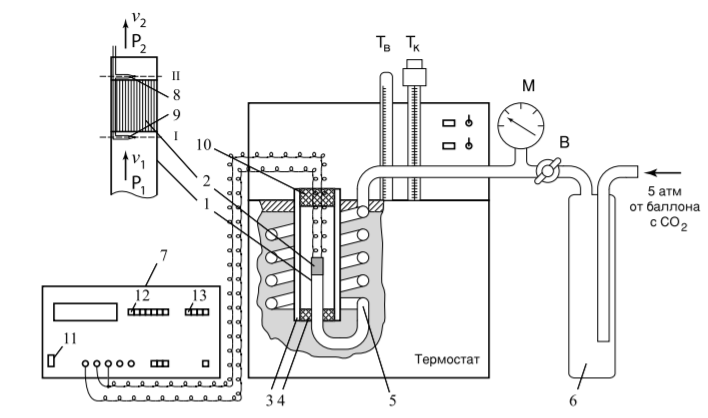
\includegraphics{Pictures/Рис 1.png}
	\caption{Схема установки для изучения эффекта Джоуля–Томсона}
\end{figure}
\noindent Это изменение температуры ничтожно мало по сравнению с измеряемым эффектом (несколько градусов).

\indent В данной лабораторной работе исследуется коэффициент дифференциального эффекта Джоуля–Томсона для углекислого газа. По экспериментальным результатам оценивается коэффициент теплового расширения, постоянные в уравнении Ван-дер-Ваальса и температура инверсии углекислого газа. Начальная температура газа $T_{1}$ задается термостатом. Измерения проводятся при трех температурах: комнатной, $30^\circ C$ и $50^\circ C.$
\\
\\
\noindent \textbf{Экспериментальная установка.} Схема установки для исследования эффекта Джоуля–Томсона в углекислом газе представлена на рисунке. Основным элементом установки является трубка 1 с пористой перегородкой 2, через которую пропускается исследуемый газ. Трубка имеет длину 80 мм и сделана из нержавеющей стали, обладающей, как известно, малой теплопроводностью. Диаметр трубки $d = 3$ мм, толщина стенок 0,2 мм. Пористая перегородка расположена в конце трубки и представляет собой стеклянную пористую пробку со множеством узких и длинных каналов. Пористость и толщина пробки $(l = 5$ мм) подобраны так, чтобы обеспечить оптимальный поток газа при перепаде давлений $\Delta P \leqslant 4$ атм (расход газа составляет около 10 см$^3$/c); при этом в результате эффекта Джоуля–Томсона создается достаточная разность температур.

\indent Углекислый газ под повышенным давлением поступает в трубку через змеевик 5 из балластного баллона 6. Медный змеевик омывается водой и нагревает медленно протекающий через него газ до температуры воды в термостате. Температура воды измеряется термометром $T_{\text{в}}$, помещенным в термостате. Требуемая температура воды устанавливается и поддерживается во время эксперимента при помощи контактного термометра $T_{\text{к}}$.

\indent Давление газа в трубке измеряется манометром М и регулируется вентилем В (при открывании вентиля В, т. е. при повороте ручки против часовой стрелки, давление $P_{1}$ Давление газа в трубке измеряется манометром М и регулируется вентилем В (при открывании вентиля В, т. е. при повороте ручки против часовой стрелки, давление $P_{2}$, то этот манометр непосредственно измеряет перепад давления на входе и на выходе трубки $\Delta P = P_{1} - P_{2}.$

\indent Разность температур газа до перегородки и после нее измеряется дифференциальной термопарой медь — константан. Константановая проволок а диаметром 0,1 мм соединяет спаи 8 и 9, а медные проволоки (того же диаметра) подсоединены к цифровому вольтметру 7. Отвод тепла через проволоку столь малого сечения пренебрежимо мал. Для уменьшения теплоотвода трубка с пористой перегородкой помещена в трубу Дьюара 3, стенки которой посеребрены, для уменьшения теплоотдачи, связанной с излучением. Для уменьшения теплоотдачи за счет конвекции один конец трубы Дьюара уплотнен кольцом 4, а другой закрыт пробкой 10 из пенопласта. Такая пробка практически не создает перепада давлений между внутренней полостью трубы и атмосферой.
\\
\\
\\
\\



\begin{center}
	\textbf{\LARGE Ход работы}
\end{center}

\begin{enumerate}
\item Перед началом работы убедимся в том, что термостат залит водой, а все электрические приборы заземлены. Следует помнить, что при используемых в работе перепадах давления ($\Delta P \leqslant 4$ атм) величина эффекта не превышает 5$^\circ C$ (200 мкВ по показаниям вольтметра), так что установка весьма чувствительна к электрическим и тепловым помехам.


\item Установим на контактном термометре $T_{\text{к}}$ температуру регулирования, близкую к комнатной, и включим термостат.

\item На вольтметре 7 выключатель «Сеть» 11 поставим в положение «Вкл». Убедимся, что на вольтметре нажаты кнопки «АВП» 12 (автоматический выбор предела) и «U=» 13 (род работы). Запишем величину показаний вольтметра при
$\Delta P = 0$ атм в таблицу 1 (они могут быть ненулевыми из-за различных паразитных ЭДС). Будем использовать эту величину для корректировки показаний вольтметра в дальнейших измерениях: $E = U(P) - U(0)$.

Откроем регулирующий вентиль В настолько, чтобы избыточное давление составило $\Delta P \approx 4$ атм.

\item Через 10–15 минут после подачи давления, когда полностью затухнут переходные процессы, запишем показания вольтметра в таблицу 1.

\item При помощи вентиля В установим давление на 0,5 атм меньше первоначального. Через 5 минут, когда установятся давление и разность температур, вновь запишем показания манометра и вольтметра в таблицу 1.

\item Проведем в сумме 6 таких измерений значений давления при комнатной температуре и запишем результаты в таблицу 1.

\begin{table}[H]
	\centering
	\begin{tabular}{|l|c|c|c|c|c|c|}
		\hline
		\multicolumn{3}{|c|}{$t = 20^\circ C$}                                & \multicolumn{4}{c|}{$U(0) = 4,0$ мкВ}  \\ \hline
		$\Delta P$, атм                         & 3,95          & 3,5         & 3,0      & 2,5     & 2,0     & 1,5     \\ \hline
		$U$, мкВ                                & -116,0        & -100,9      & -79,0    & -57,9   & -38,9   & -26,1   \\ \hline
		$\Delta U_{\pm}$, мкВ                   & -120,0        & -104,9      & -83,0    & -61,9   & -42,9   & -30,1   \\ \hline
		$\Delta T_{\pm},^\circ C$               & -2,95         & -2,58       & -2,04    & -1,52   & -1,05   & -0,74   \\ \hline
		$\Delta U = |\Delta U_{\pm}|$, мкВ      & 120,0         & 104,9       & 83,0     & 61,9    & 42,9    & 30,1    \\ \hline
		$\Delta T = |\Delta T_{\pm}|, ^\circ C$ & 2,95          & 2,58        & 2,04     & 1,52    & 1,05    & 0,74    \\ \hline
		\multicolumn{3}{|c|}{$t = 30^\circ C$}                                & \multicolumn{4}{c|}{$U(0) = -6,1$ мкВ} \\ \hline
		$\Delta P$, атм                         & 4,0           & 3,5         & 3,0      & 2,5     & 2,0     & 1,5     \\ \hline
		$U$, мкВ                                & -110,0        & -93,0       & -75,0    & -57,1   & -36,1   & -23,0   \\ \hline
		$\Delta U_{\pm}$, мкВ                   & -103,9        & -86,9       & -68,9    & -51,0   & -30,0   & -16,9   \\ \hline
		$\Delta T_{\pm},^\circ C$               & -2,50         & -2,09       & -1,66    & -1,23   & -0,72   & -0,41   \\ \hline
		$\Delta U = |\Delta U_{\pm}|$, мкВ      & 103,9         & 86,9        & 68,9     & 51,0    & 30,0    & 16,9    \\ \hline
		$\Delta T = |\Delta T_{\pm}|, ^\circ C$ & 2,50          & 2,09        & 1,66     & 1,23    & 0,72    & 0,41    \\ \hline
		\multicolumn{3}{|c|}{$t = 50^\circ C$}                                & \multicolumn{4}{c|}{$U(0) = -4,0$ мкВ} \\ \hline
		$\Delta P$, атм                         & \multicolumn{2}{c|}{4,0}    & 3,5      & 3,0     & 2,5     & 2,0     \\ \hline
		$U$, мкВ                                & \multicolumn{2}{c|}{-100,0} & -82,9    & -68,9   & -48,1   & -36,0   \\ \hline
		$\Delta U_{\pm}$, мкВ                   & \multicolumn{2}{c|}{-96,0}  & -78,9    & -64,9   & -44,1   & -32,0   \\ \hline
		$\Delta T_{\pm},^\circ C$               & \multicolumn{2}{c|}{-2,26}  & -1,86    & -1,53   & -1,04   & -0,75   \\ \hline
		$\Delta U = |\Delta U_{\pm}|$, мкВ      & \multicolumn{2}{c|}{96,0}   & 78,9     & 64,9    & 44,1    & 32,0    \\ \hline
		$\Delta T = |\Delta T_{\pm}|, ^\circ C$ & \multicolumn{2}{c|}{2,26}   & 1,86     & 1,53    & 1,04    & 0,75    \\ \hline
	\end{tabular}
\caption{}
\end{table}
При $t = 20^\circ C$ используем $\Delta T = \Delta U \cdot \frac{1}{40,7} \cdot \frac{^\circ C}{\text{В}}$;

При $t = 30^\circ C$ используем $\Delta T = \Delta U \cdot \frac{1}{41,6} \cdot \frac{^\circ C}{\text{В}}$;

При $t = 50^\circ C$ используем $\Delta T = \Delta U \cdot \frac{1}{42,5} \cdot \frac{^\circ C}{\text{В}}$.

\item Построим график $\Delta T(\Delta P)$ и по наклону определим коэффициент Джоуля-Томсона $\mu_{\text{д-т}}$ при данной температуре:


\vspace{2mm}
$\Delta T = \mu_{\text{д-т}}\Delta P$
\vspace{2mm}


Используя МНК, находим:
\vspace{2mm}

$\mu_{\text{д-т}} = 0,68 \text{ }\frac{^\circ C}{\text{атм}}$

$\sigma_{\mu_{\text{д-т}}} = 0,03 \text{ }\frac{^\circ C}{\text{атм}}$

\begin{figure}[H]
	\centering
	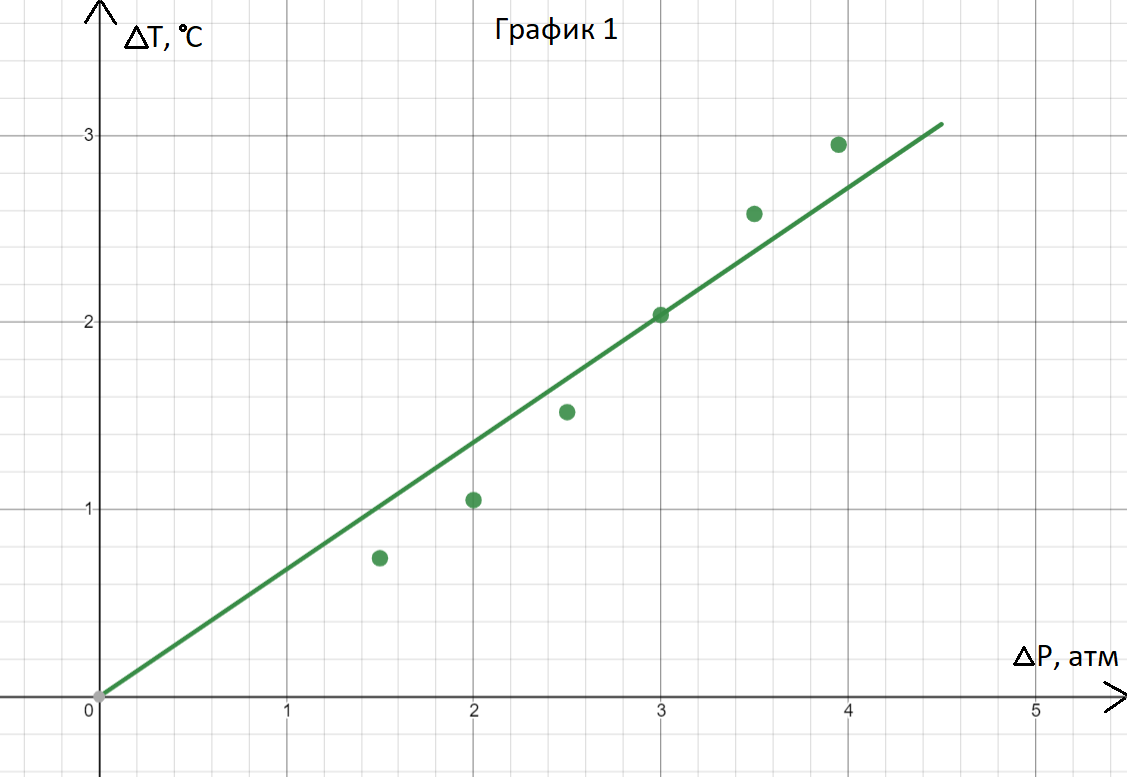
\includegraphics[scale = 0.6]{Pictures/График 1.png}
\end{figure}
\vspace{13mm}
\item Окончив измерения при комнатной температуре, закроем регулирующий вентиль В и установим на контактном термометре температуру 30$^\circ C$.

\item Когда температура установится и установка войдет в стационарный режим, повторим измерения, как указано в пунктах 3–7 и запишем результаты в таблицу 1. При обработке результатов учтем, что чувствительность термопары медь — константан зависит от температуры:

\begin{table}[H]
	\centering
	\begin{tabular}{|c|c|c|c|c|c|}
		\hline
		Температура, $^\circ C$ & 0-10  & 10-20 & 20-30 & 30-40 & 40-50  \\ \hline
		мкВ/$^\circ C$          & 38,9  & 39,8  & 40,7  & 41,6  & 42,5   \\ \hline
		Температура, $^\circ C$ & 50-60 & 60-70 & 70-80 & 80-90 & 90-100 \\ \hline
		мкВ/$^\circ C$          & 43,3  & 44,1  & 44,9  & 45,6  & 46,4   \\ \hline
	\end{tabular}
\end{table}

Строим график $\Delta T(\Delta P)$:

\vspace{2mm}
$\Delta T = \mu_{\text{д-т}}\Delta P$
\vspace{2mm}

Используя МНК, получаем:
\vspace{2mm}

$\mu_{\text{д-т}} = 0,55 \text{ }\frac{^\circ C}{\text{атм}}$

$\sigma_{\mu_{\text{д-т}}} = 0,04 \text{ }\frac{^\circ C}{\text{атм}}$

\begin{figure}[H]
	\centering
	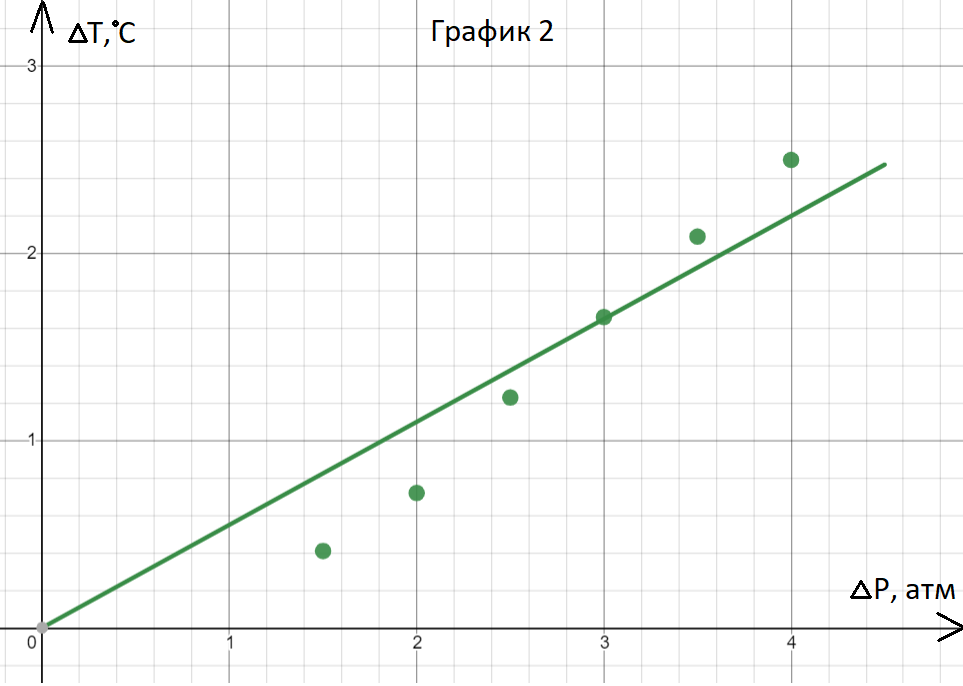
\includegraphics[scale = 0.7]{Pictures/График 2.png}
\end{figure}
\vspace{13mm}
\item Окончив измерения при 30 $^\circ C$ , проделаем такие же измерения, как указано в пунктах 3–7, для температуры 50 $^\circ C$. Результаты записываем в таблицу 1.

Строим график $\Delta T(\Delta P)$:

\vspace{2mm}
$\Delta T = \mu_{\text{д-т}}\Delta P$
\vspace{2mm}

Используя МНК, получаем:
\vspace{2mm}

$\mu_{\text{д-т}} = 0,51 \text{ }\frac{^\circ C}{\text{атм}}$

$\sigma_{\mu_{\text{д-т}}} = 0,03 \text{ }\frac{^\circ C}{\text{атм}}$

\begin{figure}[H]
	\centering
	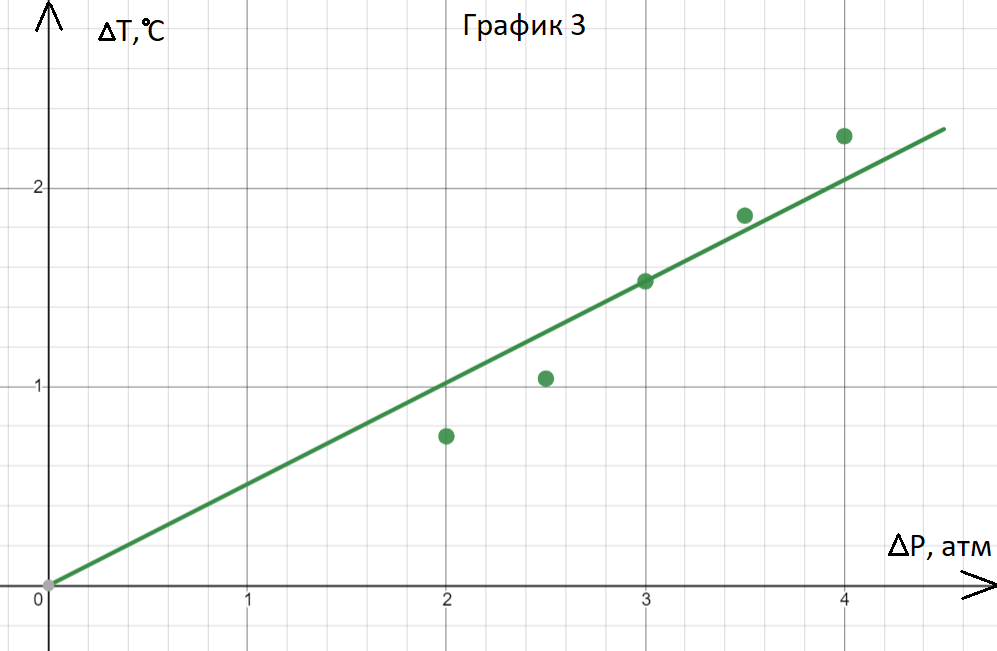
\includegraphics[scale = 0.7]{Pictures/График 3.png}
\end{figure}
\vspace{13mm}

\item Используя формулу (3) и экспериментальные данные, полученные при трех значениях температуры, определите постоянные $a$ и $b$ для углекислого газа по двум парам температур: комнатной и 30$^\circ C$, а также 30$^\circ C$ и 50$^\circ C$.

1-2):
\begin{equation*}
	\begin{cases}
		\mu_{\text{д-т}_{1}} = \frac{\frac{2a}{RT_{1}} - b}{C_{p}}
		\\
		\mu_{\text{д-т}_{2}} = \frac{\frac{2a}{RT_{2}} - b}{C_{p}}
	\end{cases}
\end{equation*}

Решая систему относительно $a$ и $b$, получаем:

\begin{equation*}
	\begin{cases}
		a = \frac{(\mu_{\text{д-т}_{1}} - \mu_{\text{д-т}_{2}})RC_{p}T_{1}T_{2}}{2(T_{2} - T_{1})}
		\\
		\\
		b = \frac{C_{p}(\mu_{\text{д-т}_{1}}T_{1} - \mu_{\text{д-т}_{2}}T_{2})}{T_{2} - T_{1}}
	\end{cases}
\end{equation*}
\\
\\

\begin{equation*}
	a = \frac{(0,68 - 0,55)\cdot 10^{-5} \cdot 8,314 \cdot 40 \cdot 293 \cdot 303}{2(303 - 293)}\frac{\text{Па}\cdot \text{м}^6}{\text{моль}^2} \approx 1,92 \text{ }\frac{\text{Па}\cdot \text{м}^6}{\text{моль}^2}
\end{equation*}
\\
\\
\begin{equation*}
		b = \frac{40 \cdot (0,68 \cdot 293 - 0,55 \cdot 303) \cdot 10^{-5}}{303 - 293}\frac{\text{м}^3}{\text{моль}} \approx 1,30 \cdot 10^{-3}\text{ }\frac{\text{м}^3}{\text{моль}}
\end{equation*}
\\
\\
\newpage
2-3):

\begin{equation*}
	\begin{cases}
		a = \frac{(\mu_{\text{д-т}_{2}} - \mu_{\text{д-т}_{3}})RC_{p}T_{2}T_{3}}{2(T_{3} - T_{2})}
		\\
		\\
		b = \frac{C_{p}(\mu_{\text{д-т}_{2}}T_{2} - \mu_{\text{д-т}_{3}}T_{3})}{T_{3} - T_{2}}
	\end{cases}
\end{equation*}
\\
\\

\begin{equation*}
	a = \frac{(0,55 - 0,51)\cdot 10^{-5} \cdot 8,314 \cdot 40 \cdot 303 \cdot 323}{2(323 - 303)}\frac{\text{Па}\cdot \text{м}^6}{\text{моль}^2} \approx 0,33 \text{ }\frac{\text{Па}\cdot \text{м}^6}{\text{моль}^2}
\end{equation*}
\\
\\
\begin{equation*}
	b = \frac{40 \cdot (0,55 \cdot 303 - 0,51 \cdot 323) \cdot 10^{-5}}{323 - 303}\frac{\text{м}^3}{\text{моль}} \approx 3,84 \cdot 10^{-5}\text{ }\frac{\text{м}^3}{\text{моль}}
\end{equation*}
\\
\\
При помощи формулы (4) и формулы $T_{\text{инв}} = \frac{27}{4}T_{\text{кр}}$ найдем температуру инверсии углекислого газа и его критическую температуру:

$T_{\text{инв}} = \frac{2a}{Rb}$

\vspace{3mm}

$T_{\text{кр}} = \frac{4}{27}T_{\text{инв}} = \frac{8}{27}\frac{a}{Rb}$

\vspace{3mm}

1-2):

$T_{\text{инв}} = \frac{2 \cdot 1,92}{8,314 \cdot 1,3 \cdot 10^{-3}}$ K $\approx 355$ K

\vspace{3mm}

$T_{\text{кр}} = \frac{8}{27}\cdot\frac{1,92}{8,314\cdot 1,3 \cdot 10^{-3}}$ K $\approx 53$ K

\vspace{10mm}

2-3):

$T_{\text{инв}} = \frac{2 \cdot 0,33}{8,314 \cdot 3,84 \cdot 10^{-5}}$ K $\approx 2067$ K

\vspace{3mm}

$T_{\text{кр}} = \frac{8}{27}\cdot\frac{0,33}{8,314\cdot 3,84 \cdot 10^{-5}}$ K $\approx 306$ K

\item Сравним полученные значения с табличными.

Видно, что результаты пары 2-3) гораздо точнее 1-2). У пары 2-3) ошибка измерения $a$ и $b$ составляет $\thicksim 10-15\%$ по сравнению с табличными значениями. Это потому, что измерения пары 2-3) проводились при температуре, что ближе к $T_{\text{кр}}$, чем пары 1-2).
\\
\\
Таким образом, точность уравнения Ван-дер-Ваальса невысока. Она описывает газы лучше, чем уравнение идеального газа, однако все еще очень неточно.
\newpage
\item Оценим ошибки измерений:
\vspace{3mm}

$a = \frac{(\mu_{\text{д-т}_{1}} - \mu_{\text{д-т}_{2}})RC_{p}T_{1}T_{2}}{2(T_{2} - T_{1})} \hspace{60mm} \sigma_{a} = \frac{RC_{p}T_{1}T_{2}}{2(T_{2} - T_{1})} \sqrt{\sigma_{\mu_{\text{д-т}_{1}}}^2 + \sigma_{\mu_{\text{д-т}_{2}}}^2}$

\vspace{3mm}

$b = \frac{C_{p}(\mu_{\text{д-т}_{1}}T_{1} - \mu_{\text{д-т}_{2}}T_{2})}{T_{2} - T_{1}}\hspace{63mm}  \sigma_{b} = \frac{C_{p}}{T_{2} - T_{1}}\sqrt{T_{1}^2\sigma_{\mu_{\text{д-т}_{1}}}^2 + T_{2}^2\sigma_{\mu_{\text{д-т}_{2}}}^2}$

\vspace{3mm}

$T_{\text{инв}} = \frac{2a}{Rb} \hspace{82.5mm} \sigma_{T_{\text{инв}}} = T_{\text{инв}}\sqrt{\left(\frac{\sigma_{a}}{a}\right)^2 + \left(\frac{\sigma_{b}}{b}\right)^2}$

\vspace{3mm}

$T_{\text{кр}} = \frac{8}{27}\frac{a}{Rb} \hspace{80mm} \sigma_{T_{\text{кр}}} = T_{\text{кр}}\sqrt{\left(\frac{\sigma_{a}}{a}\right)^2 + \left(\frac{\sigma_{b}}{b}\right)^2}$

\vspace{5mm}
1-2):


$\sigma_{a} = 0,73 \text{ }\frac{\text{Па}\cdot\text{м}^6}{\text{моль}^2}$

\vspace{3mm}

$\sigma_{b} = 0,6\cdot 10^{-3}\text{ }\frac{\text{м}^3}{\text{моль}}$

\vspace{3mm}

$\sigma_{T_{\text{инв}}} = 212$ K

\vspace{3mm}

$\sigma_{T_{\text{кр}}} = 31$ K

\vspace{7mm}

Как видим, погрешности сравнимы с самими значениями, следовательно, используемая модель достаточно плохо описывает поведение газа при данных условиях.

\vspace{5mm}

2-3):


$\sigma_{a} = 0,07 \text{ }\frac{\text{Па}\cdot\text{м}^6}{\text{моль}^2}$

\vspace{3mm}

$\sigma_{b} = 0,23\cdot 10^{-5}\text{ }\frac{\text{м}^3}{\text{моль}}$

\vspace{3mm}

$\sigma_{T_{\text{инв}}} = 310$ K

\vspace{3mm}

$\sigma_{T_{\text{кр}}} = 46$ K

\vspace{7mm}

На этот раз погрешности гораздо меньше самих значений. Они составляют $\thicksim15-20\%$ от самих результатов, что говорит о том, что используемая модель описывает газ очень неплохо при данных условиях, хотя и с ошибками.
 
\end{enumerate}
\newpage

\textbf{Вывод:} в работе было определено изменение температуры углекислого газа при протекании через малопроницаемую перегородку при разных начальных значениях давления и температуры. Также в работе были вычислены коэффициенты Ван-дер-Ваальса $a$ и $b$ для углекислого газа:

\vspace{3mm}

$a = (0,33\pm 0,07)\text{ }\frac{\text{Па}\cdot \text{м}^6}{\text{моль}^2}$

\vspace{3mm}

$b = (3,84\pm 0,23)\cdot 10^{-5}\text{ }\frac{\text{м}^3}{\text{моль}}$

\vspace{3mm}

\noindent Помимо этого была определена температура инверсии и критическая температура для углекислого газа:

\vspace{3mm}

$T_{\text{инв}} = (2067\pm 310)$ K

\vspace{3mm}

$T_{\text{кр}} = (306\pm 46)$ K. 
\end{document}
